\documentclass[sigconf, review]{acmart}


\IfFileExists{upquote.sty}{\usepackage{upquote}}{}
\IfFileExists{microtype.sty}{% use microtype if available
  \usepackage[]{microtype}
  \UseMicrotypeSet[protrusion]{basicmath} % disable protrusion for tt fonts
}{}
\makeatletter
\@ifundefined{KOMAClassName}{% if non-KOMA class
  \IfFileExists{parskip.sty}{%
    \usepackage{parskip}
  }{% else
    \setlength{\parindent}{0pt}
    \setlength{\parskip}{6pt plus 2pt minus 1pt}}
}{% if KOMA class
  \KOMAoptions{parskip=half}}
\makeatother

%%
%% This is file `sample-manuscript.tex',
%% generated with the docstrip utility.
%%
%% The original source files were:
%%
%% samples.dtx  (with options: `manuscript')
%%
%% IMPORTANT NOTICE:
%%
%% For the copyright see the source file.
%%
%% Any modified versions of this file must be renamed
%% with new filenames distinct from sample-manuscript.tex.
%%
%% For distribution of the original source see the terms
%% for copying and modification in the file samples.dtx.
%%
%% This generated file may be distributed as long as the
%% original source files, as listed above, are part of the
%% same distribution. (The sources need not necessarily be
%% in the same archive or directory.)
%%
%%
%% Commands for TeXCount
%TC:macro \cite [option:text,text]
%TC:macro \citep [option:text,text]
%TC:macro \citet [option:text,text]
%TC:envir table 0 1
%TC:envir table* 0 1
%TC:envir tabular [ignore] word
%TC:envir displaymath 0 word
%TC:envir math 0 word
%TC:envir comment 0 0
%%
%%
%% The first command in your LaTeX source must be the \documentclass command.


% Options for packages loaded elsewhere
\PassOptionsToPackage{unicode}{hyperref}
\PassOptionsToPackage{hyphens}{url}
\PassOptionsToPackage{dvipsnames,svgnames,x11names}{xcolor}

\IfFileExists{bookmark.sty}{\usepackage{bookmark}}{\usepackage{hyperref}}

%% PANDOC PREAMBLE BEGINS


\providecommand{\tightlist}{%
  \setlength{\itemsep}{0pt}\setlength{\parskip}{0pt}}\usepackage{longtable,booktabs,array}
\usepackage{calc} % for calculating minipage widths
% Correct order of tables after \paragraph or \subparagraph
\usepackage{etoolbox}
\makeatletter
\patchcmd\longtable{\par}{\if@noskipsec\mbox{}\fi\par}{}{}
\makeatother
% Allow footnotes in longtable head/foot
\IfFileExists{footnotehyper.sty}{\usepackage{footnotehyper}}{\usepackage{footnote}}
\makesavenoteenv{longtable}
\usepackage{graphicx}
\makeatletter
\def\maxwidth{\ifdim\Gin@nat@width>\linewidth\linewidth\else\Gin@nat@width\fi}
\def\maxheight{\ifdim\Gin@nat@height>\textheight\textheight\else\Gin@nat@height\fi}
\makeatother
% Scale images if necessary, so that they will not overflow the page
% margins by default, and it is still possible to overwrite the defaults
% using explicit options in \includegraphics[width, height, ...]{}
\setkeys{Gin}{width=\maxwidth,height=\maxheight,keepaspectratio}
% Set default figure placement to htbp
\makeatletter
\def\fps@figure{htbp}
\makeatother

\definecolor{mypink}{RGB}{219, 48, 122}
\makeatletter
\@ifpackageloaded{caption}{}{\usepackage{caption}}
\AtBeginDocument{%
\ifdefined\contentsname
  \renewcommand*\contentsname{Table of contents}
\else
  \newcommand\contentsname{Table of contents}
\fi
\ifdefined\listfigurename
  \renewcommand*\listfigurename{List of Figures}
\else
  \newcommand\listfigurename{List of Figures}
\fi
\ifdefined\listtablename
  \renewcommand*\listtablename{List of Tables}
\else
  \newcommand\listtablename{List of Tables}
\fi
\ifdefined\figurename
  \renewcommand*\figurename{Figure}
\else
  \newcommand\figurename{Figure}
\fi
\ifdefined\tablename
  \renewcommand*\tablename{Table}
\else
  \newcommand\tablename{Table}
\fi
}
\@ifpackageloaded{float}{}{\usepackage{float}}
\floatstyle{ruled}
\@ifundefined{c@chapter}{\newfloat{codelisting}{h}{lop}}{\newfloat{codelisting}{h}{lop}[chapter]}
\floatname{codelisting}{Listing}
\newcommand*\listoflistings{\listof{codelisting}{List of Listings}}
\makeatother
\makeatletter
\makeatother
\makeatletter
\@ifpackageloaded{caption}{}{\usepackage{caption}}
\@ifpackageloaded{subcaption}{}{\usepackage{subcaption}}
\makeatother
%% PANDOC PREAMBLE ENDS

\setlength{\parindent}{10pt}
\setlength{\parskip}{0pt}

\hypersetup{
  pdftitle={Bibat: Batteries-include Bayesian Analysis Template},
  pdfauthor={Teddy Groves},
  colorlinks=true,
  linkcolor={blue},
  filecolor={Maroon},
  citecolor={Blue},
  urlcolor={red},
  pdfcreator={LaTeX via pandoc, via quarto}}

%% \BibTeX command to typeset BibTeX logo in the docs
\AtBeginDocument{%
  \providecommand\BibTeX{{%
    Bib\TeX}}}

%% Rights management information.  This information is sent to you
%% when you complete the rights form.  These commands have SAMPLE
%% values in them; it is your responsibility as an author to replace
%% the commands and values with those provided to you when you
%% complete the rights form.
\setcopyright{acmcopyright}
\copyrightyear{2024}
\acmYear{2024}
\acmDOI{}

%% These commands are for a PROCEEDINGS abstract or paper.
\acmConference[KDD]{KDD}{Aug 25--29, 2024}{Barcelona, Esp}
\acmPrice{}
\acmISBN{}

%% Submission ID.
%% Use this when submitting an article to a sponsored event. You'll
%% receive a unique submission ID from the organizers
%% of the event, and this ID should be used as the parameter to this command.
%%\acmSubmissionID{123-A56-BU3}

%%
%% For managing citations, it is recommended to use bibliography
%% files in BibTeX format.
%%
%% You can then either use BibTeX with the ACM-Reference-Format style,
%% or BibLaTeX with the acmnumeric or acmauthoryear sytles, that include
%% support for advanced citation of software artefact from the
%% biblatex-software package, also separately available on CTAN.
%%
%% Look at the sample-*-biblatex.tex files for templates showcasing
%% the biblatex styles.
%%

%%
%% The majority of ACM publications use numbered citations and
%% references.  The command \citestyle{authoryear} switches to the
%% "author year" style.
%%
%% If you are preparing content for an event
%% sponsored by ACM SIGGRAPH, you must use the "author year" style of
%% citations and references.
%% Uncommenting
%% the next command will enable that style.
%%\citestyle{acmauthoryear}


%% end of the preamble, start of the body of the document source.
\begin{document}


%%
%% The "title" command has an optional parameter,
%% allowing the author to define a "short title" to be used in page headers.
\title{Bibat: Batteries-include Bayesian Analysis Template}

%%
%% The "author" command and its associated commands are used to define
%% the authors and their affiliations.
%% Of note is the shared affiliation of the first two authors, and the
%% "authornote" and "authornotemark" commands
%% used to denote shared contribution to the research.


  \author{Teddy Groves}
  \orcid{0000-0002-7109-3270}
            \affiliation{%
                  \institution{Danish Technical University}
                                  \city{Kongens Lyngby}
                                  \country{Denmark}
                      }


%% By default, the full list of authors will be used in the page
%% headers. Often, this list is too long, and will overlap
%% other information printed in the page headers. This command allows
%% the author to define a more concise list
%% of authors' names for this purpose.
%\renewcommand{\shortauthors}{Trovato et al.}
%%
%% The abstract is a short summary of the work to be presented in the
%% article.
\begin{abstract}
Bayesian statistical workflow offers a powerful way to learn from data,
but software software projects that implement complex Bayesian workflows
in practice are unusual, partly due to the difficulty of orchestrating
Bayesian statistical software. Bibat addresses this challenge by
providing a full-featured, scalable Bayesian statistical analysis
project using an interactive template. Bibat is available on the Python
Package index, documented at \url{https://bibat.readthedocs.io/} and
developed at \url{https://github.com/teddygroves/bibat/}. This paper
explains the motivation for bibat, briefly describes intended usage,
discusses key design choices, and reviews several examples of bibat's
use in scientific applications.
\end{abstract}

%%
%% The code below is generated by the tool at http://dl.acm.org/ccs.cfm.
%% Please copy and paste the code instead of the example below.
%%

%%
%% Keywords. The author(s) should pick words that accurately describe
%% the work being presented. Separate the keywords with commas.
\keywords{Python, Bayesian workflow, Methodology}

\begin{teaserfigure}
  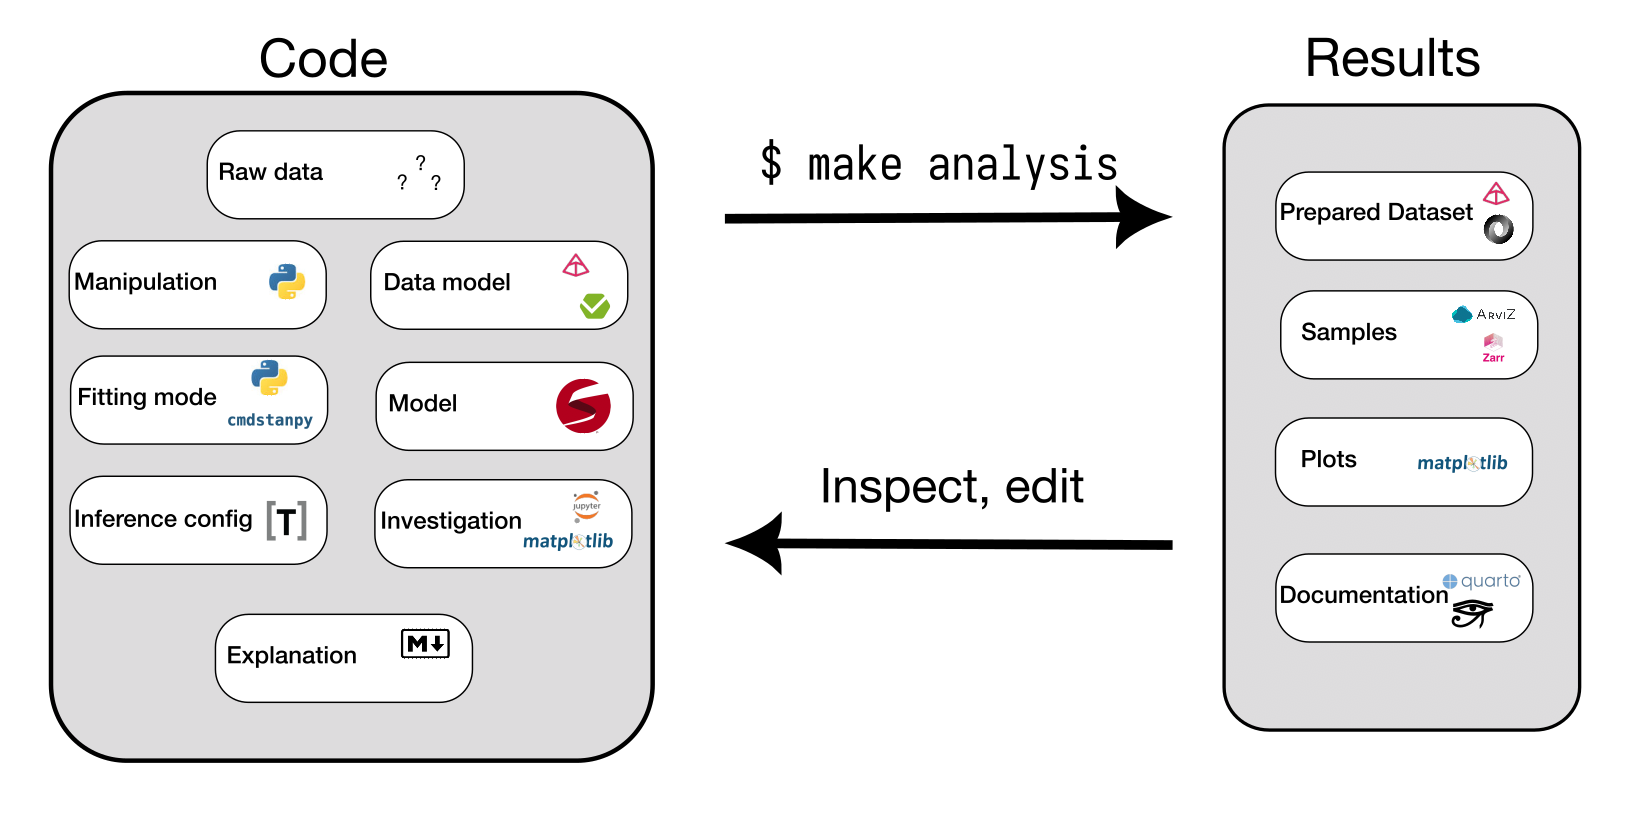
\includegraphics[width=\textwidth]{img/workflow.png}
  \caption{Schematic representation of a Bayesian workflow implemented
using bibat. The author inspects their analysis's results, edits files
corresponding to the boxes on the left, runs the command
\texttt{make\ analysis}, then repeats. Note that this workflow is
modular, accommodates plurality and results in a final analysis that can
be fully reproduced using a single command.}
  \Description{DESCRIPTION}
\end{teaserfigure}

%%
%% This command processes the author and affiliation and title
%% information and builds the first part of the formatted document.
\maketitle

\setlength{\parskip}{-0.1pt}

\section{Introduction: the problem of orchestrating Bayesian workflow
software}\label{introduction-the-problem-of-orchestrating-bayesian-workflow-software}

The idea that Bayesian statistical analysis comprises not just
inference, but also specific approaches to related activities like data
preparation, model design, diagnosis, debugging and criticism, dates at
least to \citet{boxBayesianInferenceStatistical1992}. There is
increasing scholarly recognition of the need for a holistic view of
``Bayesian workflow''
\citep{gelmanBayesianWorkflow2020, grinsztajnBayesianWorkflowDisease2021, gabryVisualizationBayesianWorkflow2019}.
Relatedly, software tools now exist that address most individual aspects
of a Bayesian workflow: see \citet{strumbeljPresentFutureSoftware} for a
review of the state of the art.

Unfortunately, currently available tools typically address one, or at
most a handful, of Bayesian workflow activities; it is left to the
individual project team to orchestrate the components. Writing software
that performs this orchestration can be time-consuming and tricky,
especially in the common scenario where it is not initially clear how
many, or what kind of, statistical models, datasets, data manipulations
or investigations an analysis will require.

Bibat addresses this difficulty by providing a full-featured,
high-quality Bayesian workflow project that can be extended to implement
a wide range of statistical analyses.

\section{How bibat works}\label{how-bibat-works}

\subsection{Installation and usage}\label{installation-and-usage}

Bibat can be installed on the Windows, linux or macos command line on by
running the command \texttt{pip\ install\ bibat} and then used by
running the command \texttt{bibat}. This command triggers an interactive
form which prompts the user to select a range of customisation options.
Bibat then creates a new directory containing code that implements an
example analysis, with customisations reflecting the user's choices.
This analysis works immediately, and can be reproduced with the single
command \texttt{make\ analysis} without the need for any further action
by the user: in this sense bibat comes with ``batteries included''.

\subsection{Documentation}\label{documentation}

Bibat is documented at \url{https://github.com/teddygroves/bibat/}. The
documentation website includes instructions for getting started, a
detailed explanation of bibat's concepts and an extended vignette
illustrating how to implement a complex statistical analysis starting
from bibat's example analysis usage. In addition, the documentation site
contains a full description of bibat's python API and command line
interface, instructions for contributing and a section discussing
accessibility considerations.

\section{Design choices}\label{design-choices}

Bibat's design was informed by these considerations.

\subsection{Accommodate a wide range of statistical
analyses}\label{accommodate-a-wide-range-of-statistical-analyses}

Bibat projects explicitly allow for plurality at the level of input
datasets, prepared datasets, statistical models, fitting modes,
computation methods and analyses. In addition, bibat ensures that there
are minimal restrictions on the kind of components: for example,
datasets need not be singular or tabular, and statistical models need
not be representable in formula syntax.

Thanks to these accommodations a project team using bibat should
typically not need to foresee the ultimate requirements of their
analysis before starting the project.

\subsection{Encourage reproducibility}\label{encourage-reproducibility}

Bibat provides a preconfigured makefile with a target \texttt{analysis}
triggering creation of an isolated environment, installation of
dependencies, data preparation, statistical computation and analysis of
results. In this way a bibat analysis can be reproduced on most
platforms using a single command.

Bibat also provides its Python code in the form of a package configured
using modern conventions for specifying dependencies and configuring
tooling, so that it is easy to maintain reproducibility as the analysis
develops.

\subsection{Use widely-adopted, open source and actively developed
tools}\label{use-widely-adopted-open-source-and-actively-developed-tools}

Bibat projects are is written in modern Python and uses pydantic
\citet{pydanticdevelopersPydantic2022} and pandera
\citep{niels_bantilan-proc-scipy-2020} for data modelling, Stan
\citep{carpenterStanProbabilisticProgramming2017} for statistical
inference, cmdstanpy \citep{standevelopmentteamCmdStanPy2022} for
python-Stan interface, arviz \citep{kumarArviZUnifiedLibrary2019} for
storing and analyzing inferences and sphinx
\citep{georgbrandlandthesphinxteamSphinx2022} and quarto
\citep{Allaire_Quarto_2022} for documentation.

Bibat itself is also written in modern Python and uses the popular tools
cookiecutter \citep{greenfeldCookiecutter2021}, pydantic and click
\citep{clickdevelopersClickPythonComposable2022}.

Bibat's makefile detects the current operating system and attempts to
install cmdstan appropriately if necessary. This functionality addresses
a common issue where researchers find it difficult to install Stan,
especially on Windows.

\subsection{Implement community standards and best practices for
collaborative software
development}\label{implement-community-standards-and-best-practices-for-collaborative-software-development}

Bibat projects include a preconfigured test environment, continuous
integration, linting and pre-commit hooks, making them suitable for
collaborative software development. In addition, including documentation
as a first class component of the analysis addresses a common problem in
academic statistics projects where the paper gets out of sync with the
code.

Bibat itself is continuously tested to ensure that it works on the
operating systems Linux, macOS and Windows. Bibat's continuous
integration runs a test suite as well as an end-to-end functional test
on all supported Python versions.

Bibat is part of the PyOpenSci ecosystem, allowing for community help
with maintenance as well as peer review for code and documentation
quality, usability and accessibility. The PyOpenSci peer review for
bibat can be found here:
\url{https://github.com/pyOpenSci/software-submission/issues/83}

\section{Challenges}\label{challenges}

This section describes some specific challenges that often affect
Bayesian workflow projects and how bibat addresses them.

\subsection{Address complexity using a modular, file based
approach}\label{address-complexity-using-a-modular-file-based-approach}

As discussed in \citet{gelmanBayesianWorkflow2020}, Bayesian workflows
are complicated, featuring plurality, cyclicity and complexity at many
levels. Bibat accommodates this by separating non-interacting analysis
components into modules and by serialising data to files wherever
possible. Prepared datasets, statistical models, inference
configurations, inference results, plots and analyses all have file
representations. Fitting modes, data manipulations and data models are
modularised in code through the use of appropriately structured data
classes and functions.

Thanks to this approach it is possible to perform small sub analyses
individually and to iteratively add components without needing to
consider everything at once.

\subsection{Fitting modes}\label{fitting-modes}

As part of a Bayesian workflow it can be necessary to fit a model and
dataset in different ways. For example, one might perform MCMC sampling
of both the prior and posterior distributions, perform multiple
leave-out-one-fold fits for cross-validation or need to compare MCMC
sampling with an optimisation-based alternative.

Bibat accommodates this need by introducing an abstraction called
``fitting mode''. This abstraction allows bibat projects to handle
fitting a model and dataset in different ways appropriately and
flexibly. For example, the provided prior sampling fitting mode creates
a Stan input dictionary with the \texttt{likelihood} data variable set
to \texttt{0}, performs MCMC sampling and writes data to the
\texttt{InferenceData} group \texttt{prior}. Bibat provides fitting
modes corresponding for prior sampling, posterior sampling and k-fold
posterior sampling. Users can easily add additional fitting modes by
copying these examples.

\section{Post launch use}\label{post-launch-use}

Bibat has been used for several real statistical analyses.

\citet{grovesteddyDgfreg2023} used bibat to compare a Bayesian and two
non-Bayesian approaches to modelling a biochemical thermodynamics
dataset. Bibat facilitated this analysis even though it was not very
large by providing the fitting mode abstraction, which was very useful
for comparing the different methods.

In \citet{grovesBaseball2022}, Bibat was used to implement a sports
analysis involving two datasets, two models and four inferences,
demonstrating that the generalised Pareto distribution can be used to
describe hitting ability in baseball. This analysis is now included in
bibat as an illustration, along with an accompanying tutorial.

\begin{figure}

\centering{

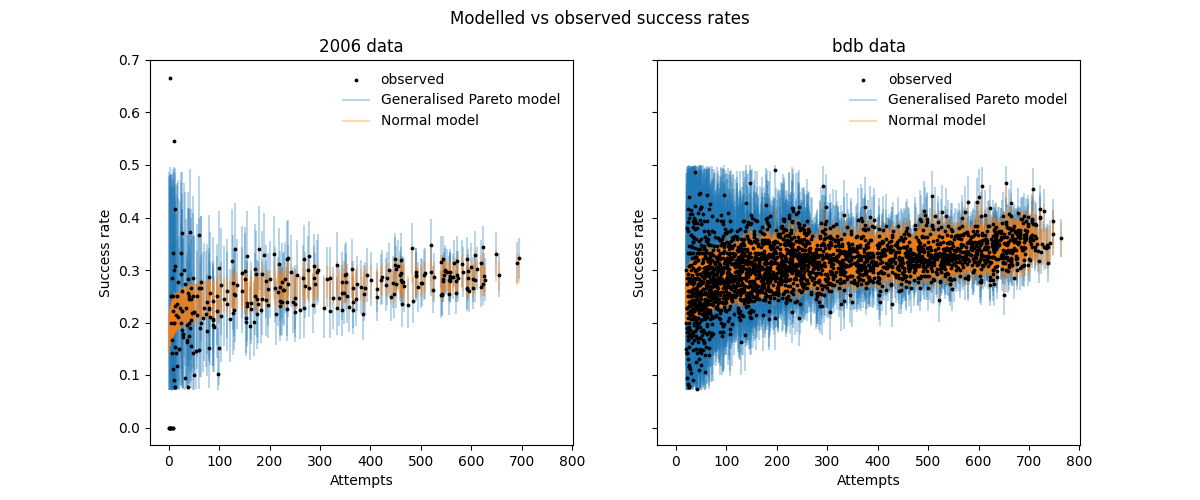
\includegraphics[width=0.5\textwidth,height=\textheight]{img/baseball.png}

}

\caption{\label{fig-baseball}A graphical posterior predictive check
produced as part of a bibat analysis that fit two statistical models to
two datasets of baseball data. The coloured lines show each model's
posterior predictive distributions and the black dots show the two
observed datasets. See
\url{https://github.com/teddygroves/bibat/tree/main/bibat/examples/baseball}
for the full analysis.}

\end{figure}%

In \citet{grovesteddySphincter2024}, bibat was used to implement an
analysis of cerebrovascular data from mice, involving two raw datasets,
6 prepared datasets, 15 models and 15 inferences. In this case bibat's
modular design made it straightforward to iteratively add data
transformations and models while maintaining reproducibility.

These cases illustrate that bibat can be useful in a variety of real
Bayesian workflows, with different sizes, subject matters and emphases.

Bibat has a growing user community, with 16 GitHub stars at the time of
writing.

\section{Comparison with alternative
software}\label{comparison-with-alternative-software}

Other than bibat, there is currently no interactive template that
specifically targets Bayesian workflow projects. There are some
templates that arguably encompass Bayesian workflow as a special case of
data analysis project, such as cookiecutter-data-science
\citep{drivendataCookiecutterdatascience2022}, but these are of limited
use compared with a specialised template due to the many specificities
of Bayesian workflow.

There is some software that addresses the general task of facilitating
Bayesian workflow, but using a different approach from bibat's. For
example, bambi \citep{capretto2020} and brms
\citep{burknerBrmsPackageBayesian2017} aim to make implementing Bayesian
workflows easier by providing ergonomic ways to specify and fit Bayesian
regression models to tabular datasets. Bibat is complementary with these
packages, as it targets use cases that they do not support, such as
analyses where complex datasets or custom models might be required.

\section{Statements and Declarations}\label{statements-and-declarations}

The authors have no financial or non-financial interests that are
directly or indirectly related to the work submitted for publication.

\bibliographystyle{ACM-Reference-Format}
\bibliography{bibliography.bib}

%% begin pandoc before-bib
%% end pandoc before-bib
%% begin pandoc biblio
%% end pandoc biblio
%% begin pandoc include-after
%% end pandoc include-after
%% begin pandoc after-body
%% end pandoc after-body

\end{document}
\endinput
%%
%% End of file `sample-manuscript.tex'.
